\begin{figure}[pos=tbp]
\centering
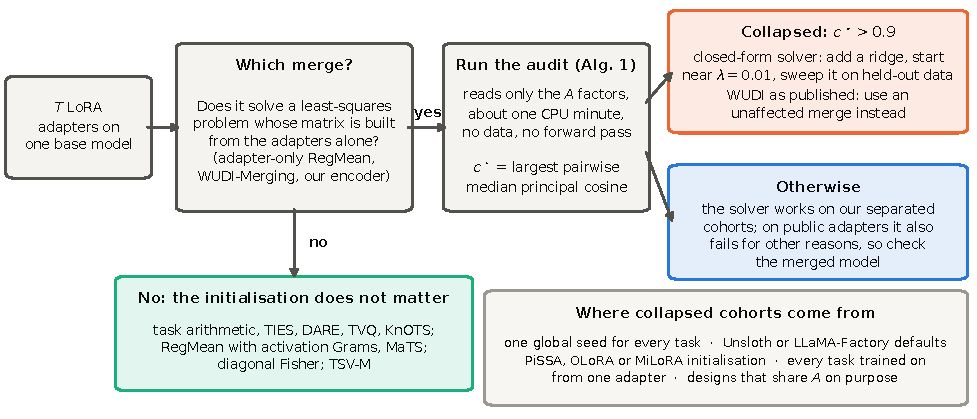
\includegraphics[width=\textwidth]{nc/figures/fig_decision.pdf}
\caption{What to do before merging a LoRA cohort, from the results of
\S\ref{sec:merging}. The audit is Algorithm~\ref{alg:audit}, and $0.9$ is its
threshold for a collapsed cohort. Only merges on the path to the right are
affected by a shared initialisation. The box at the bottom right lists the
ways a cohort becomes collapsed (\S\ref{sec:background}, \S\ref{sec:collapse}
and \S\ref{sec:prevalence}).}
\label{fig:decision}
\end{figure}

\paragraph{What to do in practice.} The results reduce to three cases
(Figure~\ref{fig:decision}).
\begin{itemize}[leftmargin=*,itemsep=1pt,topsep=2pt]
\item Some merges average or sparsify the updates, with or without aligning
  them first. Others are solvers whose matrix is built from data or is
  diagonal. For all of these, the initialisation does not matter and no action
  is needed.
\item Some merges solve a least-squares problem whose matrix is built from the
  adapters alone, as adapter-only RegMean, WUDI-Merging and our encoder do.
  Run Algorithm~\ref{alg:audit} before using them. On our own separated
  cohorts these merges work. On public cohorts, however, adapter-built solvers
  also fail for reasons unrelated to the collapse (\S\ref{subsec:open}), so
  the merged model needs checking in any case. On a collapsed cohort, add an
  isotropic ridge to the closed-form solvers, start near $\lambda = 0.01$ and
  sweep it on held-out data. Do not rely on RegMean's shipped $\alpha$. We did
  not test a repair for WUDI as published. Running it ten times longer did not
  help: its NLL got worse on three bases and stayed within noise on the fourth
  (Table~\ref{tab:wudi}). On a collapsed cohort we would therefore use one of
  the unaffected merges instead.
\item Adapters are collapsed in several common situations. Several tasks
  fine-tuned with Unsloth or LLaMA-Factory at default settings give a collapsed
  cohort, and so do tasks each trained on from one existing adapter. A PiSSA
  cohort is collapsed whatever its seeds, and OLoRA and MiLoRA start every task
  from the same $A$ in the same way. A different seed per task avoids the first
  case and not the others. Designs that share $A$ deliberately, such as
  HydraLoRA or federated LoRA with a frozen or shared $A$, are collapsed by
  construction.
\end{itemize}
The audit is needed even though a ridge repairs most of the damage. A sweep
needs held-out data and one merge per value of $\lambda$, and no
data-free rule we tested sets $\lambda$ well (\S\ref{subsec:open}). A user
who has no data for the tasks, or who runs a method at its defaults, meets the
zeros of Figures~\ref{fig:wudi} and~\ref{fig:exposure} with no warning.
The audit needs only the $A$ factors and a CPU minute. It says before any merge
whether the choice of method matters at all.

\paragraph{Predictions that failed.} Table~\ref{tab:failed} lists every
registered prediction that did not hold. Four changed what this paper claims.
Published WUDI was not protected by its optimiser, which made it the lead
result (\S\ref{subsec:wudi}). TSV-M was not exposed, so the rule is stated
for least-squares merges alone (\S\ref{subsec:results}). The collapse is
invisible on IFEval, where the instruction adapter has little skill to lose
(\S\ref{subsec:beyond}). Solver failures on public cohorts are not specific
to the collapse (\S\ref{subsec:open}). The others are explanations that did
not survive, rules for setting the ridge without data that did not work, and
three details.

\paragraph{What we cannot explain.} Three observations have no tested
explanation. First, on CLIP ViT-B/32, published WUDI merges shared cohorts
\emph{better} than independent ones, $0.454$ against $0.358$, the opposite of
its behaviour on language models (\S\ref{subsec:beyond}). The description we
give in Appendix~\ref{app:wudi-diag}, in which Adam's steps leave the row space on a
collapsed cohort, does not account for this. Second, scaling the initial $A$ by
$0.25$ leaves a cohort collapsed, yet adapter-only RegMean then does less
damage than on the independent cohort ($0.022$ against $0.071$ nats). This happens
at the same $\kappa(\bar H)$ as a cohort where it does a great deal of damage
(\S\ref{sec:theory}). That points to the amplification, rather than the
condition number, as what a solver responds to, but it rests on two cohorts.
Third, the heuristics' lean of $0.7$ points towards shared cohorts survives
every explanation we tested. The solver failures on public cohorts are in the
same position.

\paragraph{Relation to our earlier preprint.} We withdraw two
claims of our earlier preprint~\citep{pathak2026rd}. It reported that our
encoder had the lowest worst-task loss of ten methods. That advantage came
from the shared initialisation of its cohorts: on independent cohorts the
encoder beats the best baseline on one base of four. It also reported that
worst-task NLL tracks the downstream ranking of methods. With five or six
methods that correlation cannot be measured reliably, which is why every
accuracy claim here is measured in accuracy.

\paragraph{Limitations.} The controlled experiments use four base models of 7
to 9 billion parameters and four tasks. One adapter did not train properly.
In accuracy, several adapters do not beat the base model on their own
benchmark (on Llama-3.1-8B neither the GSM8K nor the code adapter does), so the
merged models contain weak members. The seed ablation, the task-count and rank
sweep and the out-of-sample test of the scalar law are on one base. The vision
replication uses one model, and DoRA was measured in geometry only. Larger
models, other architectures and other adapter types are untested. The value of
$\kappa(\bar H)$ depends on the projector model of curvature, while the
principal cosines, which carry the audit, do not. The theory is a
leading-order expansion verified numerically, not a bound. The float32 values
we report for the unregularised encoder on shared cohorts are single draws of
a randomised SVD. They move by up to $0.23$ nats between draws, and by up to
$1.1$ nats on Mistral. On Yi this is enough to move the ratio between the two
kinds of cohort across the predicted factor of two (\S\ref{sec:merging}). The
selected ridge $\lambda^\star$ was chosen on the evaluation sets it is scored
on, so the gains we report for a tuned ridge are optimistic; the fixed
$\lambda = 0.01$ is not affected. The tests on translation and IFEval, and
MaTS in accuracy, use one cohort of each kind, so they can rule out only
differences larger than their noise threshold. Training and evaluation data overlap on two tasks ($13$ to $16\%$
for instruction following and $9$ to $12\%$ for code), so absolute scores are
optimistic. Every comparison here, however, is between the two kinds of cohort
on the same data, and on the disjoint subset the ordering of methods is
unchanged in $23$ of $24$ base-by-cohort comparisons. The library reading is of
pinned versions, and defaults can change. The prevalence of $40\%$ is among
public cohorts as the sampling frame defines them, and most of the collapsed
ones are versions of one model rather than tasks one would merge
(\S\ref{subsec:public}). Finally, adapter-built solvers fail often on released
adapters for reasons we have not identified. Those failures should not be
attributed to the collapse, and such solvers should not be used on public
adapters without checking the result.
